\section{Zielsetzung}
In einem Ionenkristall können durch Dotierung mit stärker geladenen Ionen, Dipole erzeugt werden. 
In diesem Versuch wird die Anregungsenergie und die charakteristische Relaxationszeit, der Diffusion dieser 
Durch Dotierung eines Ionenkristalls mit geladenen Ionen, entstehen Dipole in 

\section{Theorie}
	\subsection{Dipole in dotierten Ionenkristallen}
		Der in diesem Versuch verwendete Ionenkrstall ist eine Kaliumbromid Probe mit einem Gitter aus Kalium-Kationen und Brom-Anionen.
		In Abbildung \ref{fig:KBr} ist eine Darstellung eines solchen Kristalles.
		\begin{figure}
			\centering
			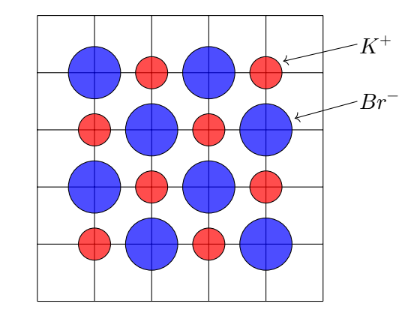
\includegraphics[]{latex/images/Kristall.PNG}
			\label{fig:KBr}
			\caption{Schematischer Aufbau des KBr Ionenkristalls.}
		\end{figure}
		Dieser Kristall wird nun mit Strontium $Sr^{2=}$ dotiert, indem einer der Kalium-Kationen ausgetauscht wird.
		Dies führt aber auch dazu, dass einer der aliegenden Kalium-Kationen so verschoben wird, dass an dessen Stelle eine Leerstelle entsteht.
		Die Leerstelle muss entstehen, damit der Kristall in Summe immernoch Ladungsneutral ist.
		Jedoch sind jetzt die vier nächsten Nachbarn negative Ladungen und die Leerstelle kann repräsentativ auch als negative Ladung betrachtet werden.
		Somit bildet jetzt die zweifach positive Dotierung mit der negativen Ladung der Leerstelle, einen Dipol. 
		Ohne vorherige Anrgeung und bei Raumtemperatur sind diese Dipole jedoch statistisch im Raum verteilt und haben somit in Summe kein Gesamtdipolmoment. 

	\subsection{Depolarisationseffekte}
		
		Ohne der Durchführung zu weit vorzugreifen, gehen wir davon aus, dass alle Dipole innerhalb des Kristalles durch eine äußere Kraft in die selbe Richtung ausgerichtet wurden und der Kristall stark abegkühlt wurde.
		Die Dipole stoßen sich aufgrund ihrer Ausrichtung gegenseitig ab, in dem Kristall ist jedoch nicht genug Energie um die Struktur des Gitters zu ändern.
		Durch aufwärmen des Kristalles können die Leerstellen genug Energie bekommen um ihre Position innerhalb des Kristall zu ändern und somit auch den Dipol zu reorientieren.
		Dises Strukturänderung innerhalb des Kristalles wird Leerstellendiffusion genannt und benötigt eine gewisse materialspezifische Aktivierungsenergie $W$.
		Da die Energieverteilung im Kristall durch die Blotzmann-Statistik $\approx\text{exp}\left(-\frac{W}{k_\text{B}T}\right)$ beschreiben wird, folgt für die Relaxationszeit:\\
		\begin{equation}
			\tau(T) = \tau_0 \text{exp}\left(\frac{-W}{k_\text{B}T}\right)
		\end{equation}
		mit der charakteristischen Relaxationszeit $\tau_0 = \tau(\infty)$.

	\subsection{Polarisationsansatz}

		Die Dipole sind in ihrem angeregtem Zustand alle in die selbe Richtung ausgerichtet.
		Dies bedeutet auch, dass durch die Relaxation im Mittel alle positiven Ladungen in 
		die gleiche Richtung verschoben werden und somit einen Strom erzeugen.
		Der Strom wird Depolarisationsstrom genannt und ist somit gleich der Änderungsrate der 
		gesamten Polarisation $P(t)$:
		\begin{equation}
			I(T) = - \frac{\text{d}P(t)}{\text{d}t}.
		\end{equation}
		Die Änderungsrate lässt sich auch mittels der Relaxationszeit darstellen und ergibt somit 
		folgende Differentialgeleichung:
		\begin{equation}
			\frac{\t{d} P(t)}{\t{d} t} = \frac{P(t)}{\tau(T)}.
			\label{eqn:diff}
		\end{equation}
		Das Lösen der Differentialgeleichung mittels Seperation der Variabeln ergibt dann:
		\begin{equation}
			P(t) = P_0 \t{exp}\left(- \frac{t}{\tau(T)} \right).
		\end{equation}
		Ableiten dieser Lösung ergibt wieder die Änderung der Polarisation und somit den 
		Depolarisationsstrom.
		\begin{equation}
			I(T) = \frac{P_0}{\tau(T)} \t{exp}\left(-\frac{t}{\tau(T)}\right)
		\end{equation}
		Hier gibt $t$ die Zeit an, die benötigt wurde um $T$ zu erreichen, 
		sie lässt sich auch als Integral schreiben:
		\begin{equation}
			I(T) = \frac{P_0}{\tau(T)} \t{exp}\left(-\int_0^t\frac{\t{d}t}{\tau(T)}\right)
			\end{equation}
		mittels einer konstanten Heizrate
		\begin{equation}
			b := \DIF{T}{t} = const
		\end{equation}
		lässt sich der Depolarisationsstrom nun als 
		\begin{equation}
			I(T) = \frac{P_0}{\tau(T)} \t{exp}\left(\frac{-1}{b\tau_0}\int_{T_0}^T\frac{\t{d}T'}{\tau(T')}\right)
		\end{equation}
		ausdrücken.

	\subsection{Stromdichtenansatz}
		
		Ein weiterer Ansatz für den Depolarisationsstrom ergibt, sich mittels der Debeye-Polarisation
		\begin{equation}
			\bar{P}(T) = \frac{N}{N_V}\frac{p^2E}{3k_\t{B}T} \, ,
		\end{equation}	
		mit dem Dipolmoment $p$, der elektrischen Feldstärke $E$, der Temperatur $T$ und der Dipoldichte $N_V$.
		Die Änderung der Anzahl der Dipole lässt sich auch hier wieder über die Relaxationszeit ausdrücken:
		\begin{equation}
			\DIF{N(T)}{t} =- \frac{N}{\tau(T)}.
		\end{equation}
		Und analog zum vorherigen Kapitel ergibt sich die Lösung der Differentialgelich zu:
		\begin{equation}
			N = N_\t{P} \t{exp}\left( \frac{-1}{b}\int_{T_0}^T \frac{\t{d}T'}{\tau(T')}\right)
		\end{equation}
		Weiterhin gilt
		\begin{align}
			I(T) = \bar{P}(T)\DIF{N}{t}& &\t{und} & & I(T) = -\bar{P}(T) \frac{N}{\tau(T)}
		\end{align}
		Zusammensetzten aller dieser Terme egibt dann einen Ausdruck für den Depolarisationsstrom
		\begin{equation}
			I(T) =\frac{p^2E}{3k_\t{B}T}\frac{N_\t{P}}{\tau_0}\t{exp}\left(\frac{-1}{b\tau_0}\int_{T_0}^T\frac{\t{d}T'}{\tau(T')}\right)\t{exp}\left(-\frac{W}{k_\t{B}T}\right).
			\label{eqn:long}
		\end{equation}		

	\subsection{Berechnung der Aktivierungsenergie $W$}
		
		\subsubsection{Bestimmung mithilfe des Maximums}

				Aufgrund der endlichen Anzahl an Dipolen entsteht trotz konstanter Heizrate, in der Theorie und im Experiment bei einer gewissen Temperatur $T_\t{max}$ ein Maximum des Depolarisationsstroms.
				Dies kann dazu genutzt werden um charakteristische Eigenschaften des Kristalles zu Bestimmen.
				Wird angenommen, dass die Aktivierungsenergie $W$ groß gegenüber der Energie $k_\t{B}T$ und der Temperaturdifferenz $T-T_0$, so wird das Integral in Gleichung \ref{eqn:long} 
				\begin{equation}
					\int_{T_0}^T\frac{\t{d}T'}{\tau(T')} \approx 0.
				\end{equation}
				Somit ergibt sich dich der Strom dann zu
				\begin{equation}
					I(T) = \frac{P^2E}{3k_\t{B}T}\frac{N_\t{P}}{\tau_0} \t{exp}\left(-\frac{W}{k_\t{B}T}\right).
				\end{equation}	
				Mittes des Logarithmus entsteht hieraus eine Geradengleichung
				\begin{equation}
					\t{ln}(I(T)) = \left(\frac{P^2EN_\t{P}}{3k_\t{B}T\tau_0}\right) - \frac{W}{k_\t{B}} \frac{1}{T}.
				\end{equation}
				Die Steigung $m$ dieser Geraden ist also $\frac{W}{k_\t{B}}$ oder
				\begin{equation}
					W = m \cdot k_\t{B}.
				\end{equation}

		\subsubsection{Verwendung des gesamten Kurvenverlaufs}

				Ein weiterer Ausdruck entsteht wenn der Verlauf der Gesamtpolarisation $P(T)$ betrachtet wird:
				\begin{equation}
					\DIF{P}{t} = \frac{P(t)}{\tau(T(t))}.
				\end{equation}
				Umstellen und mit $\DIF{T}{T}$ erweitern liefert:
				\begin{equation}
					\tau(T) = P(T) \cdot \frac{\t{d}T}{\DIF{P}{t}\t{d}T}
				\end{equation}
				Auch hier ist die Änderung der Temperatur gleich der Heizrate $b$:
				\begin{equation}
					\tau(T) = \frac{P(t)}{b}\DIF{T}{P}.
				\end{equation}
				Durch Erweitern mit $\DIF{t}{t}$ ergibt sich
				\begin{equation}
					\frac{P(t)}{b} \frac{\DIF{T}{t}}{\DIF{P}{t}}
				\end{equation}
				Die Änderung Polarisation entspricht dem Strom und mit $P = \int \t{d}P$ ist dann
				\begin{equation}
					\tau(T) = \frac{\int \DIF{P}{t}\t{d}T}{I(T)b}
				\end{equation}
				Hier kann nun erneut der Depolarisationsstrom identifiziert und eingesetzt werden:
				\begin{equation}
					\tau(T) = \frac{\int_T^\infty I(T')\t{d}T'}{I(T)b}
				\end{equation}
				und somit ergibt sich für die Aktivierungsenergie $W$:
				\begin{equation}
					W = k_\t{B}T\t{B}\left( \frac{\int_T^\infty I(T')\t{d}T'}{I(T)b\tau_0}\right)
				\end{equation}
				Die obere Grenze ist in der Praxis verschwindent da bei hohen Temperaturen keine Dipole mehr vorhanden sind, die noch relaxieren können.

	\subsection{Berechnung der charakteristischen Relaxationszeit}
				
		An dem Maximum der Stomstärke bei der Temperatur $T_\t{max}$, ist dessen Ableitung verschwindend, dies lässt sich nutzen um die charakteristische Relaxationszeit zu bestimmen.
		Dazu wird Gleichung \ref{eqn:long} nach der Temperatur abgeleitet:
		\begin{equation}
			\DIF{I(T)}{T} \approx \frac{1}{\tau_0} \left( - \frac{1}{b\tau_0}
			\int_{T_0}^T \t{exp}\left(\frac{W}{k_\t{B}T}\right)\t{d}T' - 
			\frac{W}{k_\t{B}T}\right) \cdot \left( \frac{W}{k_\t{B}T^2} - 
			\frac{1}{b\tau_0} 
			\t{exp}\left(-\frac{W}{k_\t{B}T}\right)\right).
		\end{equation}
		Dies lässt sich nun am Maximum nach der charakteristischen Relaxationszeit umstellen:
		\begin{equation}
			\tau_0 = \tau(T_\t{max})\t{exp}\left(- \frac{W}{k_\t{B}T_\t{max}}\right) = \frac{k_\t{B}T^2_\t{max}}{Wb}\t{exp}\left(-\frac{W}{k_\t{B}T_\t{max}}\right)
		\end{equation}

	
